\documentclass[11pt]{article}

\usepackage[margin=1in]{geometry}
\usepackage{amsmath,amssymb,amsthm,mathtools,bm}
\usepackage{microtype}
\usepackage{graphicx}
\usepackage{subcaption}
\usepackage[dvipsnames]{xcolor}
\usepackage[colorlinks=true,allcolors=MidnightBlue]{hyperref}
\usepackage[nameinlink,capitalise,noabbrev]{cleveref}
\usepackage[numbers,sort&compress]{natbib}
\usepackage{enumitem}

\newcommand{\R}{\mathbb R}
\newcommand{\T}{\mathbb T}
\newcommand{\E}{\mathbb E}
\newcommand{\1}{\mathbf 1}
\newcommand{\ip}[2]{\left\langle #1,#2\right\rangle}
\newcommand{\norm}[1]{\left\lVert #1\right\rVert}
\newcommand{\TV}{\operatorname{TV}}
\newcommand{\ReLU}{\operatorname{ReLU}}
\newcommand{\diag}{\operatorname{diag}}
\newcommand{\dd}{\mathrm d}
\newcommand{\cK}{\mathcal K}
\newcommand{\cL}{\mathcal L}
\newcommand{\cB}{\mathcal B}

\theoremstyle{plain}
\newtheorem{theorem}{Theorem}[section]
\newtheorem{proposition}[theorem]{Proposition}
\newtheorem{lemma}[theorem]{Lemma}
\newtheorem{corollary}[theorem]{Corollary}
\theoremstyle{definition}
\newtheorem{definition}[theorem]{Definition}
\newtheorem{assumption}[theorem]{Assumption}
\newtheorem{remark}[theorem]{Remark}

\title{\bf Dynamic Fourier Saddles Beyond the Kernel Regime:\\
Full-Training Depth, Low Rank, and Spectral-Power Descent}
\author{Anonymous Authors}
\date{}

\begin{document}
\maketitle

\begin{abstract}
We study population training on the circle for finite-depth fully connected
networks and low-rank matrix-factorized neural networks (MMNNs), in both a
right-factor-only and a full-training maximum-update scaling.  In the masked
model an exact finite-width identity factorizes the instantaneous tangent
kernel as \(K_t(x,x')=\Phi_0(x,x')G_t(x,x')\): the first-feature kernel is
fixed while a back-propagated gate kernel evolves.  In full training, every
activation and backward field evolves and must instead be closed by deep
dynamical mean-field theory (DMFT).

Our main theorem is architecture- and depth-general and does not freeze the
kernel.  At every point of a nonlinear trajectory, bounded-variation tangent
features imply \(\Lambda_{qq}(t)\leq \cB_t/q^2\).  Hence a residual
concentrated on \(\cos(qx)\) is an approximate saddle with inverse-gradient
index at least \(q^2/\cB_t\); a quantitative leakage condition gives a
quadratic residence-time lower bound.  This is a spectral regularity
obstruction, not the coordinate-support leap complexity of
\citet{abbe2023leap}: after the single input coordinate is exposed, their
leap cannot distinguish frequency four from frequency sixteen.
Layerwise, the exact tangent feature is a forward activation times a
backward field, so a mode becomes accessible only when their evolving
Fourier spectra acquire an aligned convolution channel.

We then analyze exact spectral-power descent
\(G=U\Sigma V^\top\mapsto U\Sigma^pV^\top\), including polar Muon
\((p=0)\) and Muon\({}^p\).  The update is always a strict descent direction.
Under an explicit orthogonal-sector closure, it changes the half-recovery
exponent from \(2s\) for gradient flow to
\(s(p+1)-\alpha(1-p)\) for a target spectrum \(a_q\asymp q^{-\alpha}\)
and tangent amplitudes \(q^{-s}\).  This gives a mechanism by which spectral
flattening advances a weak Fourier front.  The corresponding reused-data
Muon DMFT requires a nonseparable matrix response and Onsager memory and is
stated conditionally, not presented as an existing theorem.

Paired full-batch experiments train every block of affine-depth
\(3,5,7\) dense networks and signed low-rank MMNNs.  They confirm ordered
Fourier-sector recovery with order-one feature motion, while exact Muon and
fractional powers can move high-frequency clocks earlier on both sparse
cosine sums and power-law spectra.  The gain is optimizer-, architecture-,
and seed-dependent and is not a universal terminal-risk dominance.  Code,
raw trajectories, calibration records, and vector figures are included.
\end{abstract}

\section{Introduction}

Neural networks often fit low-frequency components before high-frequency
components.  In a fixed neural tangent kernel (NTK), the explanation is
linear: Fourier modes with smaller kernel eigenvalues decay more slowly
\citep{basri2020frequency,rahaman2019spectral}.  That explanation is
insufficient under maximum-update parameterization.  Standard and NTK
parameterizations do not retain feature learning at infinite width, whereas
\(\mu\)P does \citep{yang2021feature}.  In the rich limit the kernel evolves
with the features, and its evolution must be determined self-consistently
\citep{bordelon2022dmft}.

This raises a precise question.  Suppose the target is
\begin{equation}
 y(x)=\sum_{j=1}^J a_j\cos(q_jx),\qquad
 1\leq q_1<\cdots<q_J,
 \label{eq:target}
\end{equation}
and training displays long plateaux between the recovery of successive
modes.  Are these plateaux merely an NTK artifact, or can one establish a
hierarchy of frequency-indexed saddles in a genuinely feature-learning
limit?

The word ``leap'' requires care.  The leap complexity of
\citet{abbe2023leap} is a combinatorial measure of which new coordinates of
an isotropic high-dimensional target become detectable.  It predicts
sequential support learning and saddle-to-saddle dynamics.  It is not the
integer difference \(q_j-q_{j-1}\) between two Fourier frequencies.  The
one-dimensional periodic problem studied here has an analogous sequential
phenomenology but a different obstruction: Fourier scarcity of the tangent
features.  A major conclusion of this paper is that a universal law in the
raw difference \(q_j-q_{j-1}\) is false.  The geometric obstruction is
indexed by the absolute frequency \(q_j\).

We begin with the low-rank multi-component neural network (MMNN)
\begin{equation}
 W_2(t)=\frac{1}{\sqrt{mr}}U V(t)^\top,
 \label{eq:factorization}
\end{equation}
where \(U\in\R^{n\times r}\) is frozen and only the right factor
\(V\in\R^{m\times r}\) is trained.  The rank is extensive but low:
\(r/m\to\rho\in(0,1)\).  This distinction is essential.  If \(r\) is fixed,
the finite collection of rank channels does not self-average and there is no
deterministic DMFT without retaining channel randomness.

We then remove the mask.  Every dense matrix, both factors of every MMNN
matrix, every bias, and the readout are trained at affine depths three, five,
and seven.  This distinction matters twice.  It tests whether the saddle
hierarchy is an artifact of the frozen-left architecture, and it exposes the
optimizer question: matrix spectral descent can redistribute motion across
the singular sectors of each full gradient in a way that scalar-metric
gradient flow cannot.

Our contributions are as follows.

\begin{enumerate}[leftmargin=2em]
\item We give an exact finite-width factorization
\(K_t=\Phi_0G_t\) for right-factor training.  It isolates the DMFT order
parameter that can change: the back-propagated gate kernel \(G_t\).
\item We prove an instantaneous \(q^{-2}\) upper bound on the tangent
curvature at \emph{every} point of any finite-depth nonlinear trajectory
whose tangent features have bounded variation.  This yields a hierarchy of
approximate saddles for both masked and fully trained networks without
freezing \(K_t\).  An exact forward--backward product identity shows that
the missing Fourier supply is a convolution of the two learned spectra,
projected through rank channels in an MMNN.
\item We give a conditional residence-time theorem that remains valid for a
time-dependent, non-diagonal kernel.  Its assumptions quantify precisely the
Fourier leakage that must be checked rather than silently assuming
translation invariance after task-dependent training.
\item We prove the descent identity for a normalized singular-value power
family and, under a declared orthogonal-sector closure, derive its Fourier
front exponent for power-law targets.  We identify the matrix response that
a Muon DMFT must close and separate it from established gradient-flow DMFT.
\item We test width, depth, rank, absolute frequency, raw gap, full versus
masked training, and exact Muon powers in paired full-batch experiments.  The
masked model supplies a counterexample in which rich learning deepens
high-frequency saddles; full training and spectral flattening can reverse
the clock ordering without guaranteeing a better endpoint.
\end{enumerate}

\paragraph{Scope.}
We use ``matrix factorized'' rather than literal nonnegative matrix
factorization.  The factors are signed.  A strict nonnegative constraint
changes gradient flow into a tangent-cone or projected flow and is outside
the theorems.  We also use ``saddle'' in the quantitative approximate sense
of a state with small gradient relative to a nonzero residual; generically
these plateaux are not exact critical points.

\section{Architecture and masked \texorpdfstring{\(\mu\)P}{muP} scaling}
\label{sec:model}

Let \(\T=\R/(2\pi\mathbb Z)\), equipped with uniform probability measure.
We use the normalized inner product
\[
 \ip{u}{v}=\frac1{2\pi}\int_0^{2\pi}u(x)v(x)\dd x.
\]
The first features are
\begin{equation}
 h_j(x)=\sqrt2\,\ReLU\!\left(\cos(x-\omega_j)+b_j\right),
 \qquad j\leq m,
 \label{eq:first-features}
\end{equation}
with i.i.d. random phases and biases.  Define the rank channels, outer
preactivations, and centered output by
\begin{align}
 z_a(x,t)&=\frac1{\sqrt m}\sum_{j=1}^m V_{ja}(t)h_j(x),
 \label{eq:z}\\
 s_i(x,t)&=\frac1{\sqrt r}\sum_{a=1}^r U_{ia}z_a(x,t)+\beta_i,
 \label{eq:s}\\
 f_t(x)&=\frac1{\gamma n}\sum_{i=1}^n c_i
 \left[\phi(s_i(x,t))-\phi(s_i(x,0))\right].
 \label{eq:f}
\end{align}
Here \(U_{ia},V_{ja}(0)\sim N(0,1)\), the readouts \(c_i\in\{-1,1\}\)
are symmetric, and \(\phi=\ReLU\).  Centering makes \(f_0=0\) exactly and
removes the finite-width output fluctuation that otherwise grows as
\(\gamma\downarrow0\).  It does not alter any derivative with respect to
\(V\).

For square population loss
\begin{equation}
 \cL(V)=\frac12\norm{f_V-y}_{L^2(\T)}^2,
 \qquad R_t=f_t-y,
 \label{eq:loss}
\end{equation}
we train only \(V\) using the metric gradient flow
\begin{equation}
 \dot V(t)=-\gamma^2n\,\nabla_V\cL(V(t)).
 \label{eq:mup-flow}
\end{equation}
With \(m,n,r\) proportional, \(\gamma=\Theta(1)\) produces an order-one
change in the rank-channel fields.  This is the maximal-update scaling for
the trainable matrix, with all other layerwise learning-rate multipliers set
to zero.  We call it \emph{masked \(\mu\)P}.  It should not be confused with
full \(\mu\)P, in which every layer is trained maximally.

The scalar \(\gamma\) is the feature-learning strength used in the DMFT
parameterization of \citet{bordelon2022dmft}.  Taking the wide limit at fixed
\(\gamma>0\) gives feature learning; taking \(\gamma\downarrow0\) afterward
gives the lazy limit.  This order of limits is important.

\subsection{Full-training dense and factorized networks}
\label{sec:full-model}

The full-training controls use the periodic input embedding
\(u(x)=(\cos x,\sin x)\).  Let \(D\geq3\) denote the number of affine maps,
including the scalar readout.  A dense network is
\begin{align}
 h^1(x)&=\ReLU\!\left(Au(x)/\sqrt2+b^1\right),
 \label{eq:full-first}\\
 h^{\ell+1}(x)&=\ReLU\!\left(W^\ell h^\ell(x)/\sqrt m
 +b^{\ell+1}\right),\qquad 1\leq\ell\leq D-2,\\
 \widetilde f_\theta(x)&=m^{-1}c^\top h^{D-1}(x)+a_0,
 \qquad f_\theta(x)=\widetilde f_\theta(x)-\widetilde f_{\theta_0}(x).
 \label{eq:full-output}
\end{align}
All entries of the raw matrices and readout are initialized as standard
Gaussians.  The explicit factors \(m^{-1/2}\) in the hidden maps and
\(m^{-1}\) in the readout carry the width scaling.

For a signed low-rank MMNN, every square hidden map is replaced by
\begin{equation}
 \frac1{\sqrt m}W^\ell h
 =\frac1{\sqrt{mr}}U^\ell(V^\ell)^\top h,
 \qquad U^\ell,V^\ell\in\R^{m\times r},\quad r/m=\rho.
 \label{eq:full-factor}
\end{equation}
Both factors are trainable.  The input map, biases, and readout are also
trainable, so this is not the mask of \cref{eq:mup-flow}.  The factorization
is again signed rather than nonnegative.

Write \(\theta_\nu\) for a scalar raw parameter.  The full-training metric is
\begin{equation}
 \dot\theta_\nu=-\eta_\nu\partial_{\theta_\nu}\cL,
 \qquad
 \eta_\nu=\begin{cases}m,&\theta_\nu\neq a_0,\\1,&\theta_\nu=a_0.
 \end{cases}
 \label{eq:full-metric}
\end{equation}
This is a convenient raw-coordinate form of maximal update.  For example,
a hidden raw-matrix gradient is order \(m^{-3/2}\); multiplying it by \(m\)
gives an order \(m^{-1/2}\) entrywise change whose coherent forward action
is order one.  The input weights, hidden biases, factors, and readout obey
the analogous balance.  Width-transfer experiments check rather than assume
that the resulting feature trajectories have a common time scale.

\section{Exact dynamics and the DMFT reduction}
\label{sec:dmft}

The prediction dynamics always admit a tangent-kernel representation.  This
identity alone does not make training a kernel method: a kernel method uses a
kernel fixed independently of the trajectory, whereas the kernel below is a
state variable.

Define
\begin{align}
 \Phi_m(x,x')&=\frac1m\sum_{j=1}^m h_j(x)h_j(x'),
 \label{eq:Phi}\\
 g_a(x,t)&=\frac1{\sqrt n}\sum_{i=1}^n
 c_iU_{ia}\phi'(s_i(x,t)),
 \label{eq:g}\\
 G_{r,t}(x,x')&=\frac1r\sum_{a=1}^r g_a(x,t)g_a(x',t).
 \label{eq:G}
\end{align}

\begin{theorem}[Exact right-factor kernel factorization]
\label{thm:factorization}
At every finite width and every differentiability time of the ReLU flow,
\begin{align}
 K_t(x,x')
 &:=\gamma^2n\,\ip{\nabla_Vf_t(x)}{\nabla_Vf_t(x')}_{F}
 =\Phi_m(x,x')G_{r,t}(x,x'),
 \label{eq:kernel-factorization}\\
 \partial_tf_t(x)&=-\ip{K_t(x,\cdot)}{R_t},
 \qquad
 \dot\cL(t)=-\ip{R_t}{\mathcal K_tR_t},
 \label{eq:dissipation}
\end{align}
where \((\mathcal K_tu)(x)=\ip{K_t(x,\cdot)}{u}\).  Moreover,
\begin{equation}
 \partial_tz_a(x,t)
 =-\gamma\sqrt{\frac nr}\,
 \ip{R_t(x')\Phi_m(x,x')}{g_a(x',t)}_{x'}.
 \label{eq:z-dynamics}
\end{equation}
\end{theorem}

\begin{proof}
The chain rule gives
\[
 \frac{\partial f_t(x)}{\partial V_{ja}}
 =\frac{h_j(x)g_a(x,t)}{\gamma\sqrt{nmr}}.
\]
Multiplying the Frobenius inner product of two such gradients by
\(\gamma^2n\) and summing over \((j,a)\) yields
\eqref{eq:kernel-factorization}.  Equations \eqref{eq:dissipation} follow
from metric gradient flow.  Finally, insert the same derivative into
\eqref{eq:mup-flow}, multiply by \(h_j(x)/\sqrt m\), and sum over \(j\).
\end{proof}

Equation \eqref{eq:kernel-factorization} identifies the source of non-kernel
frequency learning.  The phase-averaged limit of \(\Phi_m\) is a stationary
first-feature kernel and is frozen.  All task-dependent adaptation enters
through \(G_{r,t}\), which records the collective outer-gate and frozen-left
factor response.  In a fully trained deep network, DMFT uses two-time
activation and gradient kernels for every layer; here the mask removes all
terms except the order parameter paired with the trained right factor.

\subsection{The extensive-rank DMFT limit}

Let
\begin{equation}
 \frac nm\to\alpha\in(0,\infty),\qquad
 \frac rm\to\rho\in(0,1],\qquad
 \frac nr\to\kappa=\frac\alpha\rho.
 \label{eq:ratios}
\end{equation}
For a finite training set and a smooth activation with polynomially bounded
derivatives, tensor-program limit theorems imply concentration of empirical
activation and gradient inner products at every finite collection of times
\citep{yang2021feature}.  The equivalent DMFT description is a
self-consistent stochastic process with two-time correlations and response
functions \citep{bordelon2022dmft}.  Applying that result to the computation
graph \eqref{eq:z}--\eqref{eq:mup-flow}, with zero learning-rate masks on the
frozen layers, gives the following specialization.

\begin{proposition}[Masked DMFT; specialization of existing wide-limit
theorems]
\label{prop:dmft}
Under the preceding hypotheses and for fixed time horizon, the empirical
order parameters \(\Phi_m\), \(G_{r,t}\), the channel covariance
\(Q_t(x,x')=r^{-1}\sum_a z_a(x,t)z_a(x',t)\), and their two-time analogues
converge in probability to deterministic limits.  Their self-consistent
single-channel process is generated by the integrated form of
\eqref{eq:z-dynamics}, together with the Gaussian frozen matrices and the
response of \eqref{eq:g} to \(z\).  The limiting prediction obeys
\begin{equation}
 \partial_tf_t=-\mathcal K_t(f_t-y),\qquad
 K_t=\Phi_0G_t,
 \label{eq:dmft-output}
\end{equation}
where \(G_t\), rather than \(G_0\), is solved self-consistently.  Finite-width
fluctuation theory for the corresponding mean-field order parameters predicts
inverse-square-root corrections away from critical amplification
\citep{bordelon2023finite}.
\end{proposition}

The proposition imports the wide-limit result; it is not a new proof of the
general tensor-program master theorem.  For ReLU, one may either use its
standard smooth approximation and pass to the limit away from zero
preactivations, or formulate convergence at almost every time.  The
finite-width identities and the Fourier theorem below require neither
Gaussianity nor a wide limit.

Equation \eqref{eq:z-dynamics} also makes the parameterization distinction
transparent.  For bounded order parameters on a fixed time interval,
\(z(t)-z(0)=O(\gamma)\); hence \(G_t-G_0\to0\) as \(\gamma\to0\).  At fixed
\(\gamma=\Theta(1)\), the prefactor
\(\gamma\sqrt{n/r}=\gamma\sqrt\kappa\) is order one.  Narrower extensive
bottlenecks therefore strengthen the field response, but this does not
determine its sign in any Fourier direction.

\begin{remark}[Why fixed rank is different]
If \(r=O(1)\), \(G_{r,t}\) remains an average of finitely many random channel
processes.  It need not converge to a deterministic kernel even if
\(m,n\to\infty\).  Fixed-rank experiments are meaningful, but their theory
is a random finite-channel mean-field process, not 
\cref{prop:dmft}.
\end{remark}

\section{A non-kernel hierarchy of Fourier saddles}
\label{sec:theory}

Let \(e_q(x)=\sqrt2\cos(qx)\), so that \(\norm{e_q}=1\).  Let
\(\theta=(\theta_\nu)_{\nu\leq P}\) collect any finite set of trained scalar
parameters and let \(M=\diag(\eta_1,\ldots,\eta_P)\succ0\) be its gradient
metric.  Thus \(M=\gamma^2nI\) for the masked model and \(M\) is given by
\cref{eq:full-metric} for full training.  We write
\(\norm{v}_M^2=v^\top Mv\).  Define
\begin{align}
 K_t(x,x')&=\nabla_\theta f_t(x)^\top M\nabla_\theta f_t(x'),
 \qquad
 \chi_{\nu,t}(x)=\sqrt{\eta_\nu}\,\partial_{\theta_\nu}f_t(x),
 \label{eq:generic-tangent}\\
 \Lambda_{q\ell}(t)
 &=\ip{e_q}{\mathcal K_te_\ell}
 =\nabla_\theta\ip{f_t}{e_q}^\top
 M\nabla_\theta\ip{f_t}{e_\ell}.
 \label{eq:fourier-matrix}
\end{align}
For the masked architecture, the generic tangent feature reduces exactly to
\begin{equation}
 \chi_{ja,t}(x)=\gamma\sqrt n\,
 \frac{\partial f_t(x)}{\partial V_{ja}}
 =\frac{h_j(x)g_a(x,t)}{\sqrt{mr}}.
 \label{eq:tangent-feature}
\end{equation}
This matrix need not be diagonal.  Although the initialization law is
translation invariant, the target \eqref{eq:target} breaks translation
symmetry during feature learning.  Treating the Fourier modes as exact
eigenfunctions of \(K_t\) would therefore smuggle a kernel-regime assumption
into the argument.

For off-diagonal statements below, the index \(\ell\) ranges over the
complete normalized real Fourier basis
\(\{1,\sqrt2\cos(kx),\sqrt2\sin(kx):k\ge1\}\); the symbol \(q\) is shorthand
for its cosine element \(\sqrt2\cos(qx)\).  Thus the leakage term includes
constant and sine components created by a finite random network.

\begin{assumption}[Finite tangent variation at a plateau]
\label{ass:BV}
For almost every time under consideration, each periodic function
\(\chi_{\nu,t}\) is of bounded variation and
\begin{equation}
 \cB_t:=\frac1{2\pi^2}\sum_{\nu=1}^P
 \TV(\chi_{\nu,t})^2<\infty.
 \label{eq:variation-budget}
\end{equation}
\end{assumption}

For a finite ReLU network this holds generically whenever the outer
preactivations have finitely many transversal zero crossings.  The value of
\(\cB_t\) is allowed to change by order one; that freedom is precisely what
keeps the result outside the NTK regime.

\begin{theorem}[Instantaneous dynamic Fourier-saddle bound]
\label{thm:dynamic-saddle}
Under \cref{ass:BV}, at every differentiability time and for every \(q\ge1\),
\begin{equation}
 0\leq\Lambda_{qq}(t)\leq\frac{\cB_t}{q^2}.
 \label{eq:q2-curvature}
\end{equation}
If \(R_t=Ae_q\), then
\begin{equation}
 \norm{\nabla_\theta\cL(\theta_t)}_{M}^2
 =A^2\Lambda_{qq}(t)
 \leq\frac{A^2\cB_t}{q^2}.
 \label{eq:gradient-bound}
\end{equation}
Consequently the inverse-gradient saddle index
\begin{equation}
 \mathsf S_q(t):=\frac{\norm{R_t}^2}
 {\norm{\nabla_\theta\cL(\theta_t)}_{M}^2}
 \label{eq:saddle-index}
\end{equation}
satisfies \(\mathsf S_q(t)\ge q^2/\cB_t\).
\end{theorem}

\begin{proof}
For a periodic bounded-variation function \(u\), integration by parts in
the Riemann--Stieltjes sense gives
\[
 \left|\ip{u}{e_q}\right|
 =\left|\frac{\sqrt2}{2\pi q}\int_0^{2\pi}\sin(qx)\,\dd Du(x)\right|
 \leq\frac{\sqrt2}{2\pi q}\TV(u).
\]
By \eqref{eq:generic-tangent},
\(\Lambda_{qq}=\sum_\nu|\ip{\chi_{\nu,t}}{e_q}|^2\).  Squaring the last
display and summing proves \eqref{eq:q2-curvature}.  If \(R_t=Ae_q\), metric
gradient flow and \eqref{eq:dissipation} give
\(\norm{\nabla_\theta\cL}_{M}^2=A^2\Lambda_{qq}\).  The saddle-index bound
follows.
\end{proof}

\begin{corollary}[Finite-depth full-training networks]
\label{cor:full-depth}
At every generic differentiability time, \cref{thm:dynamic-saddle} applies
to the fully trained dense and factorized networks
\eqref{eq:full-first}--\eqref{eq:full-factor} at every finite affine depth
and finite width.
\end{corollary}

\begin{proof}
On each activation cell, every forward field is a finite linear combination
of restrictions of trigonometric functions, and every backward field is a
finite product of such fields with ReLU gate indicators.  At a generic
parameter value no preactivation vanishes identically on a nontrivial
interval and all zero crossings are finite and transversal.  Forward
fields, gate indicators, their finite products, and therefore all tangent
features have bounded variation.  Signed factorization changes the finite
linear combinations but not this closure property.
\end{proof}

The theorem is deliberately instantaneous.  It permits \(K_t\), its
Fourier matrix, the gates, and \(\cB_t\) all to evolve.  A residence-time
claim additionally needs control of off-diagonal transport.

\begin{remark}[Wide-limit qualification]
Finite-width bounded variation does not by itself imply
\(\sup_m\cB_t^{(m)}<\infty\) for a sequence of widening networks.  If the
maximal-update sequence obeys this uniform regularity bound on a fixed time
interval, then \eqref{eq:q2-curvature} passes immediately to every limiting
DMFT curvature.  Establishing that bound from the full two-time DMFT is a
separate problem: generic finite-network BV is not a substitute for it.  Our
main-width diagnostics measure \(\Lambda_{qq}\) directly and retain
high-frequency decay, while width transfer supports a shared training scale;
neither observation proves uniform control of the larger variation budget.
\end{remark}

\begin{assumption}[Plateau purity and Fourier leakage]
\label{ass:leakage}
On a time interval \(I=[t_0,t_1]\), a next mode \(q\) satisfies
\begin{equation}
 \left|\sum_{\ell\neq q}\Lambda_{q\ell}(t)R_\ell(t)\right|
 \leq\varepsilon\Lambda_{qq}(t)|R_q(t)|,
 \qquad
 \sup_{t\in I}\cB_t\leq\cB_*,
 \label{eq:leakage}
\end{equation}
where \(R_\ell=\ip{R}{e_\ell}\) and \(0\leq\varepsilon<1\).
\end{assumption}

\begin{theorem}[Residence time with a dynamic, non-diagonal kernel]
\label{thm:residence}
Under \cref{ass:leakage}, if \(|R_q|\) decreases from \(A\) to \(B<A\)
while the trajectory remains in \(I\), then
\begin{equation}
 t_1-t_0\geq
 \frac{q^2}{(1+\varepsilon)\cB_*}\log\frac AB.
 \label{eq:residence}
\end{equation}
\end{theorem}

\begin{proof}
Project \(\partial_tR=-\mathcal K_tR\) on \(e_q\).  By
\eqref{eq:leakage} and \cref{thm:dynamic-saddle},
\[
 |\partial_tR_q|
 \leq(1+\varepsilon)\Lambda_{qq}|R_q|
 \leq(1+\varepsilon)\frac{\cB_*}{q^2}|R_q|.
\]
Integrating the logarithmic derivative proves the claim.
\end{proof}

\begin{corollary}[Dynamic saddle bound in a feature-learning DMFT limit]
\label{cor:dmft-saddle}
Consider a sequence of widths for which the maximal-update prediction and
tangent curvatures converge on a fixed time interval to the
Bordelon--Pehlevan DMFT solution.  If
\(\sup_{m,t}\cB_t^{(m)}\leq\overline{\cB}<\infty\), then the limiting,
generally time-dependent curvature satisfies
\begin{equation}
 \Lambda_{qq}^{\rm DMFT}(t)\leq\frac{\overline{\cB}}{q^2}.
 \label{eq:dmft-saddle-bound}
\end{equation}
If the limiting Fourier leakage satisfies \cref{ass:leakage}, with
\(\cB_*\) replaced by \(\overline{\cB}\), then its residence-time bound is
\eqref{eq:residence}.
\end{corollary}

\begin{proof}
Apply \cref{thm:dynamic-saddle} at each finite width and pass to the
curvature limit.  The residence statement follows by the projected residual
argument of \cref{thm:residence}.
\end{proof}

\begin{corollary}[Hierarchy and the meaning of a frequency leap]
\label{cor:hierarchy}
Suppose the modes in \eqref{eq:target} become successively residual-dominant,
and \cref{ass:leakage} holds with common \(\varepsilon,\cB_*\) on their
plateaux.  Then the lower bound on the \(j\)th residence time is proportional
to \(q_j^2\).  If \(q_{j-1}\) is held fixed, a larger raw gap implies a larger
bound.  Without fixing \(q_{j-1}\), no law depending only on
\(q_j-q_{j-1}\) follows.
\end{corollary}

This is the rigorous content of ``the bigger the frequency leap, the bigger
the saddle.''  The statement is correct when ``leap'' means the absolute new
frequency, or when the predecessor is fixed.  A translation of both
frequencies by the same integer preserves their gap but changes the bound.

\subsection{Why coordinate leap complexity does not supply this hierarchy}

The similar saddle-to-saddle phenomenology should not obscure a mismatch of
complexity measures.  The formal setting of \citet{abbe2023leap} is a
tensor-product Hermite or Fourier--Walsh basis on isotropic high-dimensional
data, not the continuous Fourier basis on \(\T\).  Even in the closest
one-coordinate Hermite analogue, the higher degree is not the next leap.

\begin{proposition}[One-coordinate leap collapse]
\label{prop:leap-collapse}
Let
\(
 h(z)=\sum_{j=1}^J a_j\operatorname{He}_{q_j}(z_1)
\)
with nonzero coefficients and distinct positive degrees.  Under
Definition~1 of \citet{abbe2023leap},
\begin{equation}
 \operatorname{Leap}(h)=\min_j q_j.
 \label{eq:leap-collapse}
\end{equation}
In particular,
\(\operatorname{He}_1+\operatorname{He}_4+\operatorname{He}_{16}\) has
leap one; the framework assigns no new coordinate leap to degrees four and
sixteen.
\end{proposition}

\begin{proof}
Whichever basis element appears first in an admissible ordering introduces
the only active coordinate, counted with its Hermite multiplicity.  Once
coordinate one belongs to the accumulated support, every later basis
element introduces zero unused coordinates under the set-difference rule.
The maximum increment for an ordering is therefore the degree of its first
element, and minimizing over orderings gives \eqref{eq:leap-collapse}.
\end{proof}

Our Fourier saddle bound is thus a \emph{within-coordinate regularity cost}.
For a genuinely high-dimensional periodic target, coordinate support
discovery and within-support oscillation can coexist.  A plausible composite
complexity would retain the coordinate leap for discovering a new support
and attach a Fourier-regularity budget to the new sector.  Neither factor is
a theorem-level substitute for the other.

\section{What DMFT adds beyond the theorem}
\label{sec:mechanism}

Theorems \ref{thm:dynamic-saddle} and \ref{thm:residence} identify a
geometric obstruction but do not prescribe the trajectory of \(\cB_t\) or
\(\Lambda(t)\).  DMFT supplies that missing dynamics through \(G_t\).
Combining \eqref{eq:kernel-factorization} with
\eqref{eq:fourier-matrix} gives
\begin{equation}
 \Lambda_{q\ell}(t)
 =\int_{\T^2}e_q(x)\Phi_0(x,x')G_t(x,x')e_\ell(x')
 \,\dd\mu(x)\dd\mu(x').
 \label{eq:dmft-fourier}
\end{equation}
There are two non-kernel escape channels.

\begin{enumerate}[leftmargin=2em]
\item \emph{Diagonal amplification:} gate motion increases
\(\Lambda_{qq}(t)\), spending more tangent-variation budget at the missing
frequency.
\item \emph{Off-diagonal transfer:} task adaptation creates
\(\Lambda_{q\ell}(t)R_\ell(t)\) large enough to violate
\cref{ass:leakage} and feed mode \(q\) from other residual components.
\end{enumerate}

Neither channel has a fixed sign.  The same gate rearrangement can align
features with a low-frequency component while removing high-frequency zero
crossings, thereby reducing \(\Lambda_{qq}\) for large \(q\).  The
right-factor-only mask is especially restrictive: \(V\) can move the gates,
but the first dictionary, left factor, and readout cannot rotate to repair a
harmful redistribution.  This predicts the suppression observed in
\cref{sec:experiments}.

For full training, the corresponding statement is layerwise.  Suppressing
normalization constants, introduce the two-time forward and backward order
parameters
\begin{align}
 C^\ell_{t,s}(x,x')
 &=\lim_{m\to\infty}\frac1m
 \ip{h_t^\ell(x)}{h_s^\ell(x')}_{\R^m},\nonumber\\
 D^\ell_{t,s}(x,x')
 &=\lim_{m\to\infty}\frac1m
 \ip{b_t^\ell(x)}{b_s^\ell(x')}_{\R^m}.
 \label{eq:deep-order-parameters}
\end{align}
where \(b_t^\ell\) is the width-normalized back-propagated field, together
with the causal responses of each field to its effective Gaussian drive.  At
equal times the dense tangent kernel has the schematic layer decomposition
\begin{equation}
 K_t(x,x')=K_t^{\rm readout+bias}(x,x')+
 \sum_{\ell}a_\ell
 C^{\ell-1}_{t,t}(x,x')D^\ell_{t,t}(x,x'),
 \label{eq:deep-kernel-order-parameters}
\end{equation}
where the positive constants \(a_\ell\) are fixed by the maximal-update
metric.  The factorized network augments this finite list with left- and
right-channel covariances and responses.  Bordelon--Pehlevan DMFT closes
these objects as coupled causal Volterra processes.  Consequently
\begin{equation}
 \dot r_q(t)=-\sum_{\ell'}
 \Lambda_{q\ell'}[C,D,\mathcal R](t)r_{\ell'}(t)
 \label{eq:deep-dmft-fourier}
\end{equation}
is nonlinear through the order parameters even though it is linear in the
instantaneous residual.  A frequency plateau is the interval during which
this self-consistent process has not supplied diagonal curvature or
off-diagonal transfer to the missing sector.  This is the DMFT content of
the feature-learning explanation; replacing \([C,D,\mathcal R](t)\) by its initial
value would reduce it to NTK dynamics.

\subsection{The exact source of Fourier supply}

The preceding ``supply'' has a concrete layerwise meaning.  Use the complex
basis \(\varphi_q(x)=e^{iqx}\), and let \(b_i^{\ell+1}(x,t)\) denote the
derivative of the output with respect to the preactivation of unit \(i\)
after the hidden matrix \(W^\ell\).

\begin{proposition}[Exact forward--backward Fourier supply]
\label{prop:fourier-supply}
In the raw maximal-update coordinates of \cref{eq:full-metric}, the
normalized tangent feature of a dense hidden weight is
\begin{equation}
 \chi_{ij,t}^{W^\ell}(x)
 =\sqrt m\,\partial_{W^\ell_{ij}}f_t(x)
 =b_i^{\ell+1}(x,t)h_j^\ell(x,t).
 \label{eq:forward-backward-product}
\end{equation}
Consequently its Fourier coefficient is the convolution
\begin{equation}
 \widehat\chi_{ij,t}^{W^\ell}(q)
 =\sum_{k\in\mathbb Z}
 \widehat b_i^{\ell+1}(k,t)\widehat h_j^\ell(q-k,t),
 \qquad
 \Lambda_{qq}^{W^\ell}(t)
 =\sum_{i,j}\left|\widehat\chi_{ij,t}^{W^\ell}(q)\right|^2.
 \label{eq:fourier-supply-convolution}
\end{equation}
The analogous identities for a factorized map are
\begin{align}
 \chi_{ia,t}^{U^\ell}(x)
 &=r^{-1/2}b_i^{\ell+1}(x,t)
   \big[(V^\ell)^\top h^\ell(x,t)\big]_a,\nonumber\\
 \chi_{ja,t}^{V^\ell}(x)
 &=r^{-1/2}h_j^\ell(x,t)
   \big[(U^\ell)^\top b^{\ell+1}(x,t)\big]_a.
 \label{eq:factorized-fourier-supply}
\end{align}
\end{proposition}

\begin{proof}
Differentiating \(W^\ell h^\ell/\sqrt m\) with respect to
\(W^\ell_{ij}\), and multiplying by the metric factor \(\sqrt m\), gives
\eqref{eq:forward-backward-product}.  The Fourier product formula gives the
first identity in \eqref{eq:fourier-supply-convolution}; summing its squared
coefficient over the block gives its tangent-curvature contribution.
Differentiating
\(U^\ell(V^\ell)^\top h^\ell/\sqrt{mr}\) with respect to each factor and
again multiplying by \(\sqrt m\) gives
\eqref{eq:factorized-fourier-supply}.
\end{proof}

These are finite-width identities, not a Gaussian or kernel approximation.
They show that a high mode \(q\) is weak when the current
forward and backward spectra contain few well-aligned pairs whose
frequencies sum to \(q\).  Learning lower modes changes both spectra and can
therefore create a new convolution channel, rotate a low-rank channel into
alignment, or destroy one.  Writing
\begin{equation}
 \dot r_q=-\underbrace{\Lambda_{qq}r_q}_{\text{diagonal supply}}
 -\underbrace{\sum_{\ell\ne q}\Lambda_{q\ell}r_\ell}_{\text{transport supply}}
 \label{eq:supply-decomposition}
\end{equation}
makes the plateau criterion explicit: both supplies are small compared with
the unresolved residual.  A feature-learning transition is the
self-consistent growth of either term through
\eqref{eq:fourier-supply-convolution}--\eqref{eq:factorized-fourier-supply}.
The \(q^{-2}\) theorem limits the diagonal route under uniform regularity;
the leakage assumption limits the transport route.  This is why the
hierarchy can persist while the tangent kernel changes by order one.

Deep linear DMFT gives analytic examples in which feature learning
accelerates power-law training \citep{bordelon2025deep}.  Data-dependent
fixed-point kernels can likewise outperform their lazy counterparts when
all relevant feature degrees of freedom adapt \citep{lauditi2025adaptive}.
Those results do not imply monotone acceleration for a masked nonlinear
architecture.  Our experiment is a counterexample to that extrapolation.

The equilibrium analysis of \citet{barbier2026statphys} is complementary.
It uses replicas and Harish--Chandra--Itzykson--Zuber (HCIZ) integrals to
describe Bayes-optimal specialization transitions in proportional-width
teacher--student networks, and it predicts metastable unspecialized
solutions.  HCIZ is not required for \eqref{eq:dmft-fourier}: we condition on
the frozen \(U\), study gradient-flow dynamics rather than an equilibrium
posterior, and never integrate a learned rotational degree of freedom.  That
work motivates the language of specialization and metastability, but using
its static free energy as a training-time potential here would be
unjustified.

\section{Spectral-power descent and the Muon front}
\label{sec:muon}

Muon replaces the singular values of a matrix gradient while preserving its
singular frames \citep{jordan2024muon}.  To isolate this operation from
momentum, weight decay, and an approximate Newton--Schulz polynomial, we use
the exact memoryless map.  For a matrix block \(B\in\R^{d_o\times d_i}\)
with gradient \(G_B=U\Sigma V^\top\), define
\begin{equation}
 \Psi_p(G_B)=U\Sigma^pV^\top,
 \qquad
 \Phi_p(G_B)=\sqrt{d_od_i}\,
 \frac{\Psi_p(G_B)}{\norm{\Psi_p(G_B)}_F},
 \qquad 0\leq p\leq1.
 \label{eq:muon-map}
\end{equation}
Zero singular values remain zero.  The member \(p=0\) is the compact polar
factor; fractional members are Muon\({}^p\) \citep{dong2026muonp}.  The RMS
normalization makes a width-independent learning rate plausible in a
maximal-update scaling; it is not, by itself, a proof of hyperparameter
transfer \citep{zhao2026principled}.  Vectors and scalar biases retain the
metric gradient update.  Up to scale, \(U\Sigma^pV^\top\) maximizes linear
descent under a Schatten-\((1+1/p)\) constraint
\citep{dong2026muonp}; polar Muon is the operator-norm endpoint.

\begin{proposition}[Exact descent identity]
\label{prop:muon-descent}
For every nonzero matrix gradient and \(p\in[0,1]\),
\begin{equation}
 \ip{G_B}{\Phi_p(G_B)}_F
 =\sqrt{d_od_i}\,
 \frac{\sum_{j:\sigma_j>0}\sigma_j^{p+1}}
 {(\sum_{j:\sigma_j>0}\sigma_j^{2p})^{1/2}}>0.
 \label{eq:muon-descent}
\end{equation}
Consequently the continuous block update
\(\dot B=-\eta_B\Phi_p(G_B)\), combined with metric descent on nonmatrix
blocks, strictly decreases the loss away from a stationary point.
\end{proposition}

\begin{proof}
Unitary invariance of the Frobenius inner product gives
\(\ip{U\Sigma V^\top}{U\Sigma^pV^\top}_F
=\sum_j\sigma_j^{p+1}\).  Substitution of the normalization in
\eqref{eq:muon-map} proves the identity.  Summing
\(\ip{\nabla_B\cL}{\dot B}_F\) over blocks gives strict dissipation.
\end{proof}

The descent identity does not say which Fourier sector advances.  That
requires an alignment statement between function-space sectors and matrix
singular vectors.  The next closure is exact when stated and deliberately
strong; the experiments measure its failures through signed mode velocity
and event coverage.

\begin{assumption}[Orthogonal singular-sector closure]
\label{ass:singular-sectors}
On a time interval, one active matrix block has residual coordinates
\(r_q=\ip{f-y}{e_q}\) and coefficient Jacobians
\begin{equation}
 J_q:=\nabla_B\ip{f}{e_q}=c_q u_qv_q^\top,
 \qquad
 u_q^\top u_\ell=v_q^\top v_\ell=\1\{q=\ell\},
 \label{eq:sector-jacobian}
\end{equation}
with \(c_q>0\).  Other blocks and cross-sector forcing are negligible.
During the half-recovery interval, the common normalization
\begin{equation}
 Z_p(t)=\frac{(\sum_\ell|r_\ell(t)c_\ell|^{2p})^{1/2}}
 {\eta_B\sqrt{d_od_i}}
 \label{eq:sector-normalization}
\end{equation}
is bounded above and below by positive constants independent of \(q\).
\end{assumption}

\begin{theorem}[Conditional Muon\texorpdfstring{\({}^p\)}{p} sector clock]
\label{thm:muon-front}
Under \cref{ass:singular-sectors}, the exact residual dynamics are
\begin{equation}
 \dot r_q=-\frac{c_q^{p+1}}{Z_p(t)}
 \operatorname{sign}(r_q)|r_q|^p.
 \label{eq:muon-sector-ode}
\end{equation}
For \(0\leq p<1\), the time to reduce \(|r_q|\) from \(a_q\) to
\(a_q/2\) is, up to the two uniform bounds on \(Z_p\),
\begin{equation}
 T_{1/2,q}^{(p)}\asymp
 c_q^{-(p+1)}a_q^{1-p}
 \frac{1-2^{p-1}}{1-p}.
 \label{eq:muon-half-time}
\end{equation}
For \(p=1\), the corresponding clock is
\(T_{1/2,q}^{(1)}\asymp c_q^{-2}\log2\).  Therefore, if
\(c_q\asymp q^{-s}\) and \(a_q\asymp q^{-\alpha}\),
\begin{equation}
 T_{1/2,q}^{(p)}\asymp
 q^{s(p+1)-\alpha(1-p)},\quad p<1,
 \qquad
 T_{1/2,q}^{(1)}\asymp q^{2s}.
 \label{eq:muon-front-exponent}
\end{equation}
\end{theorem}

\begin{proof}
Under \eqref{eq:sector-jacobian},
\(G_B=\sum_qr_qc_qu_qv_q^\top\) is already an SVD up to the signs of
\(r_q\).  Pairing \(-\Phi_p(G_B)\) with \(J_q\) gives
\eqref{eq:muon-sector-ode}.  Integrating
\(\dd |r_q|/|r_q|^p\), and bounding \(Z_p(t)\) above and below, gives
\eqref{eq:muon-half-time}.  Substitution of the two power laws yields
\eqref{eq:muon-front-exponent}.  The \(p=1\) case is the logarithmic limit.
\end{proof}

For bounded-variation tangent features, \(c_q\) is the Frobenius amplitude
of a coefficient Jacobian and \(c_q^2\) is its block curvature.  Saturation
of the Fourier bound corresponds to \(s=1\); faster decay has \(s>1\).  In
the saturated ideal closure, gradient flow has a quadratic half-error
front, while \(p<1\) reduces the exponent and also gives relatively more
motion to small-amplitude target modes.  This is the precise sense in which
Muon can shorten a Fourier leap.  It is not unconditional: different modes
need not occupy orthogonal singular frames, the normalization is global,
several blocks compete, and a spectral update may initially move a
coefficient in the wrong direction through cross-mode forcing.
More explicitly, relative to the gradient-flow exponent,
\begin{equation}
 2s-\big[s(p+1)-\alpha(1-p)\big]
 =(1-p)(s+\alpha)>0,\qquad p<1,
 \label{eq:muon-exponent-gain}
\end{equation}
so every nontrivial spectral flattening advances the asymptotic front under
the closure.  The strict inequality belongs to the closure, not to arbitrary
finite networks.

The \(p=1\) member of \eqref{eq:muon-map} is block-normalized gradient
descent, not literally the unnormalized maximal-update gradient flow used in
the baseline.  Under the uniform bound on \(Z_1\), normalization changes a
common clock prefactor but not its \(q^{2s}\) exponent.  Direct scalar-metric
gradient flow gives \(\dot r_q=-\eta c_q^2r_q\) under the same sector closure
and therefore the same frequency exponent.

For the experimental spectrum $a_q\asymp q^{-1.25}$ and the saturated
regularity value $s=1$, the ideal closure predicts clock exponents
$-.25,.50,1.25$ for $p=0,1/3,2/3$, respectively, compared with $2$ for
gradient flow.  The negative polar exponent is not a claim that harder
frequencies are intrinsically easier: a relative-error threshold shrinks
with $a_q$, and the conclusion relies on bounded common normalization and
singular-sector alignment.  The measured front is therefore compared with
this ordering, not forced to equal these ideal numbers.

\subsection{What a Muon DMFT must contain}

Full-training gradient-flow DMFT closes a two-time activation correlation
and backward response at every layer \citep{bordelon2022dmft}.  Replacing a
linear matrix-gradient update by \eqref{eq:muon-map} changes the response
channel itself.  For a full-row-rank block, let
\(S=GG^\top\) and \(b=(p-1)/2\), so that the unnormalized map is
\(\Psi_p(G)=S^bG\).  Its exact Fr\'echet derivative is
\begin{equation}
 D\Psi_p(G)[\Delta]
 =D(S^b)[G\Delta^\top+\Delta G^\top]G+S^b\Delta,
 \label{eq:frechet-muon}
\end{equation}
where \(D(S^b)\) is the Loewner divided-difference operator.  Differentiating
the normalization additionally projects out the radial component,
\begin{equation}
 D\Phi_p(G)[\Delta]
 =\frac{\sqrt{d_od_i}}{\norm{\Psi_p}_F}
 \left(D\Psi_p[\Delta]
 -\Psi_p\frac{\ip{\Psi_p}{D\Psi_p[\Delta]}_F}
 {\norm{\Psi_p}_F^2}\right).
 \label{eq:frechet-normalized}
\end{equation}

This nonseparable matrix derivative enters the retarded response or Onsager
reaction.  A reused-data Muon DMFT must therefore close layerwise two-time
correlations and responses together with the evolving singular law and a
matrix-valued memory kernel.  The three-layer program of
\citet{aiad2026sequential} derives this finite response interface and reports
earlier Hermite-sector clocks, but explicitly leaves the joint reused-data
DMFT closure conditional.  Our use is equally limited: the exact finite
descent law and \cref{thm:muon-front} are proved, whereas the self-averaging
Muon process is a physics closure tested by width transfer.  Calling the
ordinary spectral update AMP would be incorrect because it contains no
self-consistent Onsager subtraction.

\section{Experiments}
\label{sec:experiments}

We use the exact architecture in \cref{sec:model} on a uniform periodic grid
and explicit full-batch gradient descent, with no momentum, adaptive
preconditioner, or stochasticity.  The primary hierarchy has
\((q_j)=(1,4,8,16)\), amplitudes \((1,.65,.45,.30)\), width \(m=n=256\),
and rank ratio \(\rho=.25\).  Rich runs use \(\gamma=1\); lazy controls use
\(\gamma=10^{-4}\).  The Euler step is \(5\), well below the initial
linear-stability limit, and trajectories run to gradient-flow time
\(25{,}000\).  Unless noted otherwise, uncertainty is the standard
deviation over three initializations.

The instantaneous Fourier matrix is computed without forming a sample-space
kernel.  For each mode we differentiate its output coefficient and evaluate
\eqref{eq:fourier-matrix}.  This diagnostic includes the \(\mu\)P metric.
The experiments comprise hierarchy, frequency, fixed-gap, rank, width, and
spectrum controls.  Every trajectory and plotting command is released with
the paper.

\begin{figure}[t]
 \centering
 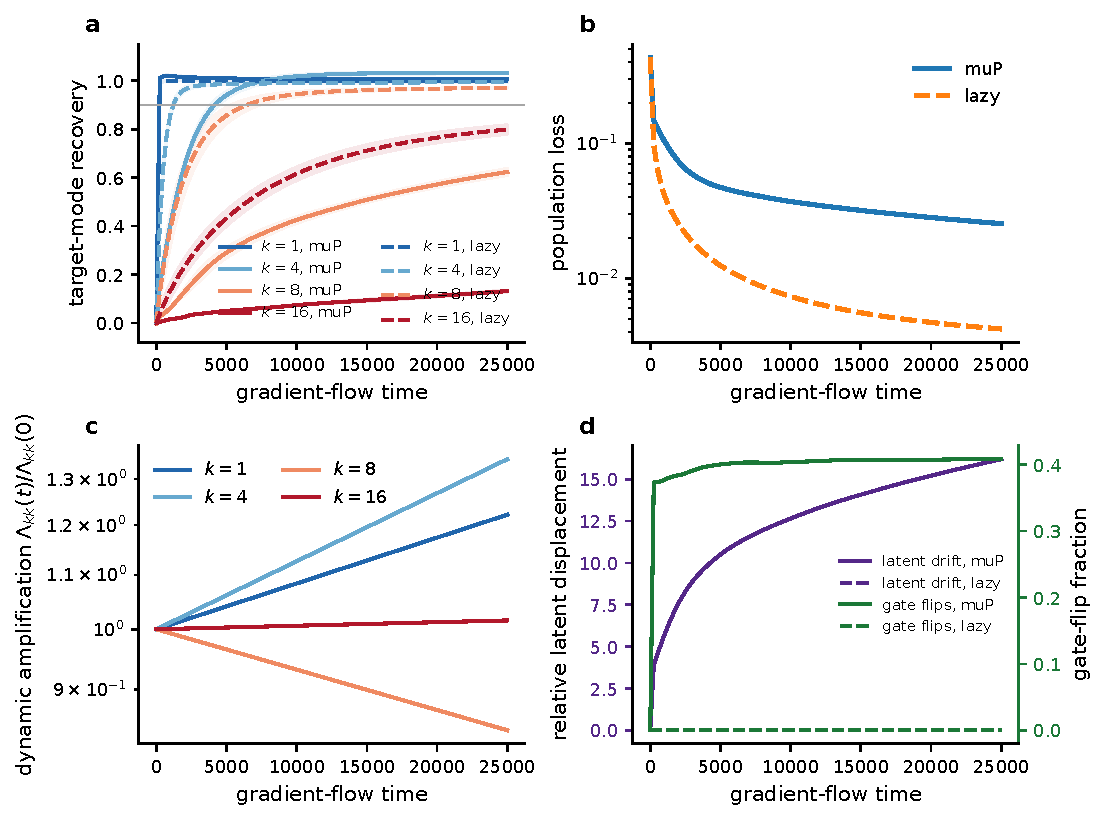
\includegraphics[width=\textwidth]{figures/hierarchy_and_kernel_evolution.pdf}
 \caption{\textbf{Hierarchical recovery with order-one feature learning.}
 (a) Fourier recovery for the sum of four cosines; solid curves are masked
 \(\mu\)P and dashed curves are lazy.  (b) Population loss.  The lazy control
 learns the high modes faster in this masked architecture.  (c) Rich-regime
 tangent-curvature renormalization.  The kernel changes non-uniformly across
 frequencies, so the trajectory is not described by \(K_0\).  (d) Latent
 displacement (left axis) and gate flips (right axis).  Curves show means
 over three seeds.}
 \label{fig:hierarchy}
\end{figure}

Figure \ref{fig:hierarchy} demonstrates the central separation.  The rich
model is manifestly non-kernel: its latent representation moves by
\(3.35\pm0.08\) initial latent norms in the post-\(q=1\) spectrum experiment,
and \(35.7\%\pm1.3\%\) of outer gates change state.  The lazy values are
\(3.13\times10^{-4}\) and \(9.2\times10^{-5}\), respectively.  Yet the
mode-recovery ordering remains low to high.

\begin{figure}[t]
 \centering
 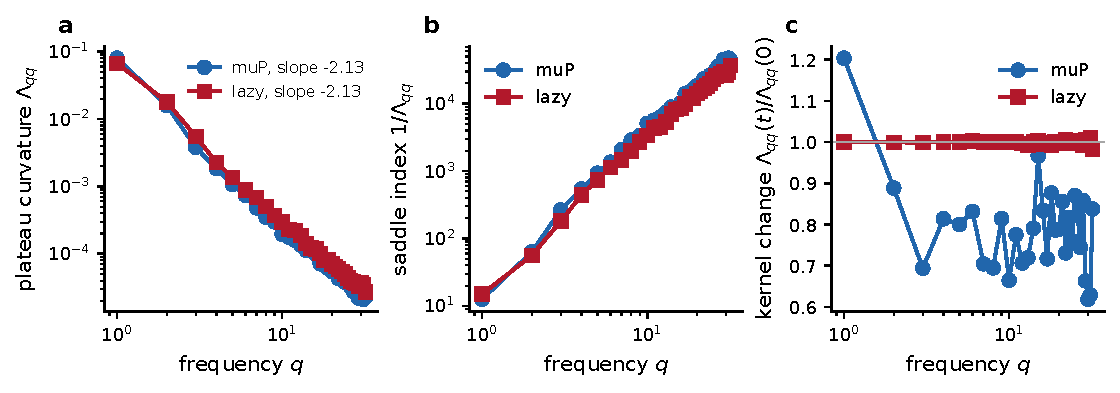
\includegraphics[width=\textwidth]{figures/dynamic_saddle_spectrum.pdf}
 \caption{\textbf{A hierarchy of dynamic Fourier saddles after fitting
 \(k=1\).}  (a) Instantaneous curvature.  Fits over \(q\ge3\) give exponents
 \(-2.13\) in both regimes.  (b) The inverse-curvature saddle index grows
 approximately quadratically.  (c) Rich feature learning changes the kernel
 by order one and frequency-selectively, whereas the lazy kernel stays at
 initialization.  Means over three seeds are shown.}
 \label{fig:spectrum}
\end{figure}

After fitting the first mode to loss below \(3.2\times10^{-7}\), the rich
curvature obeys \(\Lambda_{qq}\propto q^{-2.132}\) over \(q\ge3\); the lazy
exponent is \(-2.134\).  Thus the exponent is a geometric regularity effect,
not evidence of a frozen kernel.  The prefactor is dynamic: relative to
initialization, rich training multiplies the curvature at
\(q=1,4,8,16,32\) by approximately
\(1.20,0.81,0.69,0.83,0.84\), while lazy ratios remain near one.  The full
Fourier matrix has off-diagonal Frobenius ratio \(0.136\) in the rich regime,
confirming that exact diagonalization should not be assumed.

\begin{figure}[t]
 \centering
 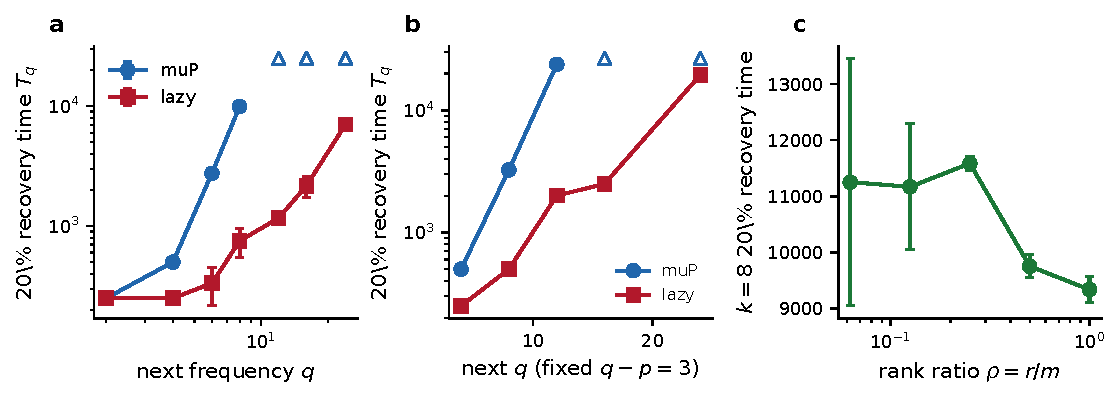
\includegraphics[width=\textwidth]{figures/frequency_rank_controls.pdf}
 \caption{\textbf{Frequency, gap, and rank controls.}
 (a) Time to recover \(20\%\) of the next mode when the predecessor is fixed
 at \(p=1\).  Unreached rich-regime modes are right-censored at the horizon
 and omitted from the connecting line.  (b) The raw gap is held exactly at
 three while both frequencies are translated: difficulty still grows with
 the absolute next frequency.  Open triangles denote censoring.  (c) Rank
 ratio changes the \(k=8\) time scale but not the existence of the hierarchy;
 error bars show one standard deviation over three seeds.}
 \label{fig:controls}
\end{figure}

For targets \(\cos x+0.5\cos(qx)\), rich \(20\%\)-recovery times at
\(q=2,4,6,8\) are approximately \(250,500,2750,9917\); modes
\(q\ge12\) do not reach the threshold by time \(25{,}000\).  The lazy
baseline reaches \(q=24\) near time \(7000\).  This does not contradict
\cref{thm:dynamic-saddle}: rich dynamics decrease the relevant high-frequency
curvatures, increasing the effective plateau constant.  Holding the raw gap
at three while translating the pair verifies that the difficulty is not a
function of the gap alone.

Rank ratios from \(.0625\) to \(1\) change the mean \(q=8\) recovery time
from roughly \(11{,}250\) to \(9{,}333\), with non-monotone finite-width
variation at intermediate ratios.  We therefore do not claim that low rank
by itself creates sequential learning or that there are exactly \(r\)
plateaux.  Rank changes the DMFT response strength and finite-channel noise;
Fourier regularity creates the saddle hierarchy.

\begin{figure}[t]
 \centering
 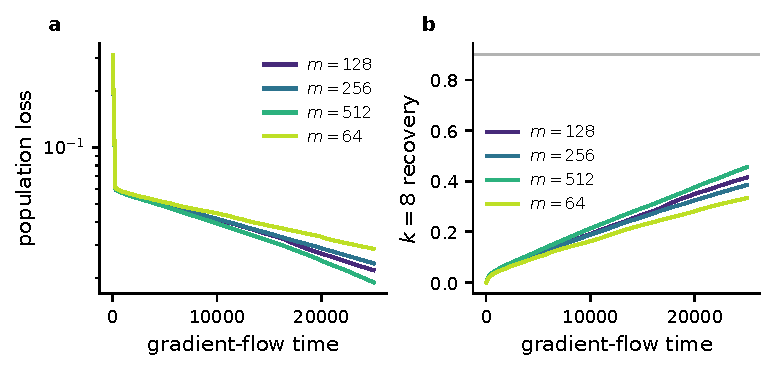
\includegraphics[width=.76\textwidth]{figures/mup_width_collapse.pdf}
 \caption{\textbf{Width consistency in masked \(\mu\)P.}  Population loss and
 \(k=8\) recovery for \(m=n\in\{64,128,256,512\}\), with
 \(r/m=.25\).  The curves approach a common rich-regime trajectory rather
 than shifting their time scale with width.}
 \label{fig:width}
\end{figure}

The width comparison in \cref{fig:width} supports the extensive-rank DMFT
interpretation.  It is not, by itself, a proof of convergence, and the
remaining deviations are compatible with the \(O(m^{-1/2})\) fluctuation
theory of \citet{bordelon2023finite}.

\subsection{Full training across depth and architecture}
\label{sec:full-experiments}

The second campaign uses the models of \cref{sec:full-model}.  Every
parameter block is trained.  The population grid has 128 points, the main
width is 128, MMNN rank ratio is \(.25\), and affine depths are
\(D\in\{3,5,7\}\).  The sparse target retains frequencies
\((1,4,8,16)\).  A second target has the power-law spectrum
\begin{equation}
 y_{\rm PL}(x)=\sum_{q=1}^{24}q^{-1.25}\cos(qx).
 \label{eq:powerlaw-target}
\end{equation}
We define the sector event as the first stored step at which
\(|\widehat f_q-a_q|/|a_q|\leq1/2\).  Unreached events are right-censored at
the common horizon.

Learning rates are selected separately for architecture, depth, and
optimizer on seeds 101 and 102, which are absent from confirmation.  The
prespecified candidate set is \(\{.1,.3,1\}\) for maximal-update gradient
descent and \(\{.003,.01,.03\}\) for every spectral power.  The calibration
score averages log relative sector error and uses log endpoint loss only as
a light tie breaker.  Confirmation uses eight paired seeds.  Spectral
updates use a direct compact SVD of each matrix gradient (the accurate
\texttt{gesvd} driver on CUDA), with relative numerical-rank threshold
$10^{-7}$; vectors and biases use metric descent.
There is no momentum, weight decay, minibatch noise, or Newton--Schulz
approximation.  Thus this is a mechanism experiment rather than a claim
about every implementation marketed as Muon.  Training and spectral
factorization use single precision throughout; this is why the direct-SVD
backend audit is part of the acceptance criteria rather than an
implementation footnote.

Calibration selected dense gradient-descent rate $.3$ at all three depths
and dense spectral rate $.01$ for all three powers.  For the MMNN it selected
gradient-descent rates $.3,.3,.1$ at depths three, five, and seven and
spectral rate $.003$ for all three powers.  Width controls reuse the
depth-five rate verbatim.
Throughout, ``earlier'' means fewer calibrated full-batch updates.  A direct
SVD is substantially more expensive per update than gradient descent; the
experiment makes no wall-clock acceleration claim.

\begin{figure}[t]
 \centering
 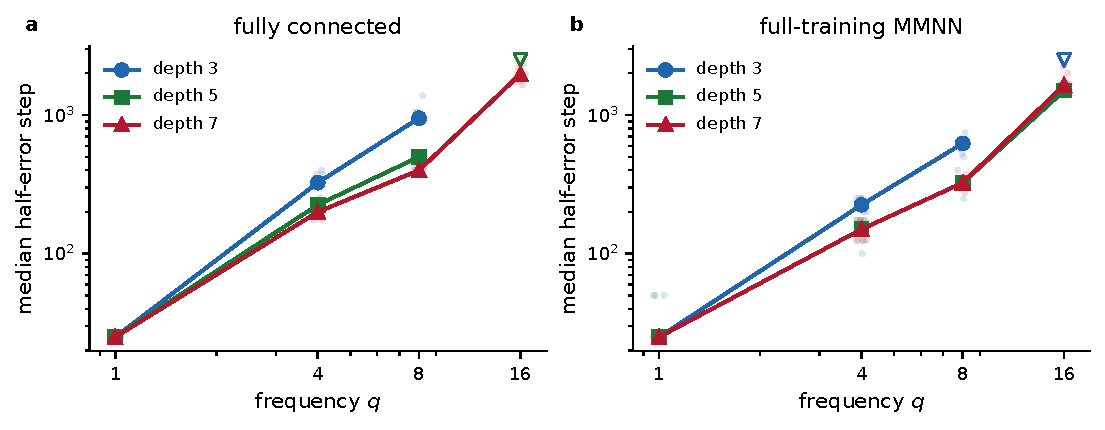
\includegraphics[width=\textwidth]{figures/full_training_depth_hierarchy.pdf}
 \caption{\textbf{The Fourier hierarchy survives full training and depth.}
 Median half-error steps under maximal-update gradient descent for affine
 depths three, five, and seven.  The left panel is fully connected; the
 right panel trains both factors of every signed low-rank MMNN map.  Open
 downward triangles denote a median that is right-censored at the training
 horizon.  The ordered clock is present across architectures, while depth
 changes its prefactor and event coverage.}
 \label{fig:full-depth}
\end{figure}

Figure~\ref{fig:full-depth} rules out the frozen-left mask as the source of
the hierarchy.  Dense and factorized networks both display successively
later sector events while every forward and backward field changes.  The
claim is deliberately not that deeper is always slower: depth changes the
variation budget, cross-mode transfer, and conditioning, so curves may cross.

At depth five the dense median half-error steps are $25,225,500$, with the
$q=16$ median censored at $2500$; the full-training MMNN gives
$25,150,325,1500$.  Median maximum hidden-feature displacement is $5.65$ and
$8.63$ initial-feature norms, respectively.  Meanwhile the mean curvature
slope over $q\geq4$ moves from $-2.02$ to $-2.34$ in the dense network and
from $-2.03$ to $-1.31$ in the MMNN, while the $q\geq4$ curvatures grow by
roughly two or more orders of magnitude.  Thus feature learning can reshape
both slope and prefactor; what persists is a decreasing high-frequency
supply, not a frozen or universal fitted exponent.
The non-kernel diagnostic is not confined to depth five: median maximum
feature displacement across depths three, five, and seven is
$3.24,5.65,10.91$ for the dense network and $5.25,8.63,10.02$ for the
MMNN.  At every one of these six architecture--depth combinations, at least
one Fourier curvature changes by a factor exceeding \(e^{4.8}\).

\begin{figure}[t]
 \centering
 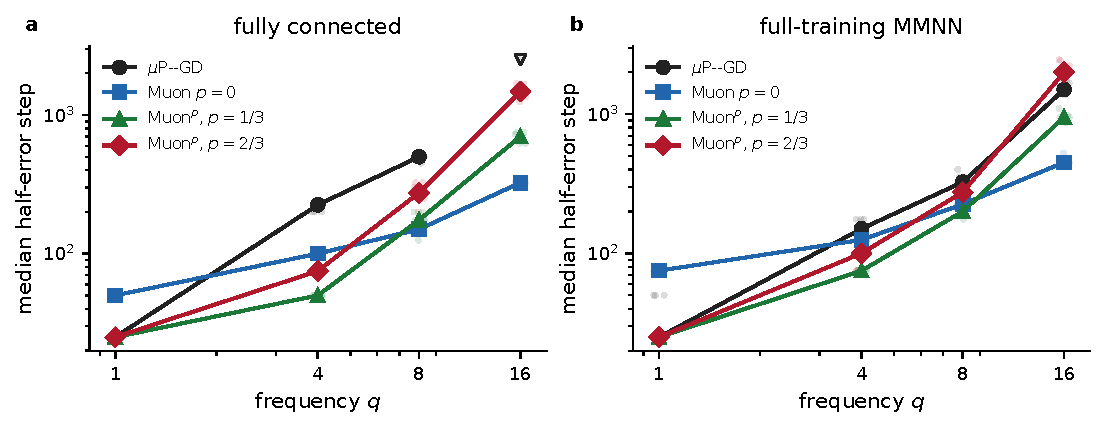
\includegraphics[width=\textwidth]{figures/muon_hierarchy_clocks.pdf}
 \caption{\textbf{Spectral powers move sparse-target sector clocks.}
 Median half-error steps at affine depth five for maximal-update gradient
 descent, polar Muon, and Muon\({}^p\) with \(p=1/3,2/3\).  Optimizers are
 calibrated on disjoint seeds and compared on paired initializations.
 Open downward triangles mark a right-censored median at the common horizon.
 Earlier crossings do not imply lower terminal risk or complete event
 coverage.}
 \label{fig:muon-clocks}
\end{figure}

\begin{figure}[t]
 \centering
 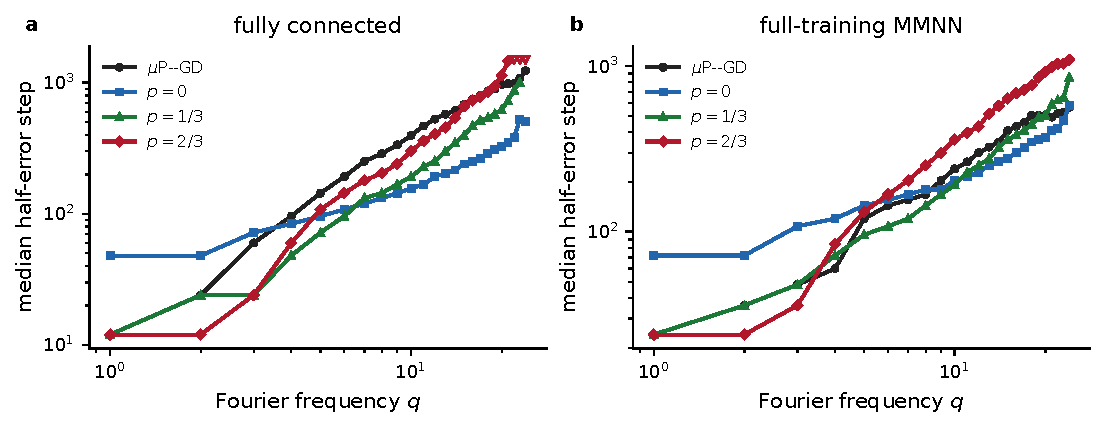
\includegraphics[width=\textwidth]{figures/muon_powerlaw_front.pdf}
 \caption{\textbf{Muon reshapes a power-law Fourier front.}
 Median half-error step for every component of
 \eqref{eq:powerlaw-target}.  Polar flattening reduces the descriptive front
 slope in both architectures, but absolute clocks, event coverage, and the
 best power are architecture-dependent.  Fractional powers can advance
 intermediate sectors while delaying or censoring the last ones. Open
 downward triangles mark right-censored medians; no high-frequency event is
 imputed.}
 \label{fig:muon-powerlaw}
\end{figure}

\begin{figure}[t]
 \centering
 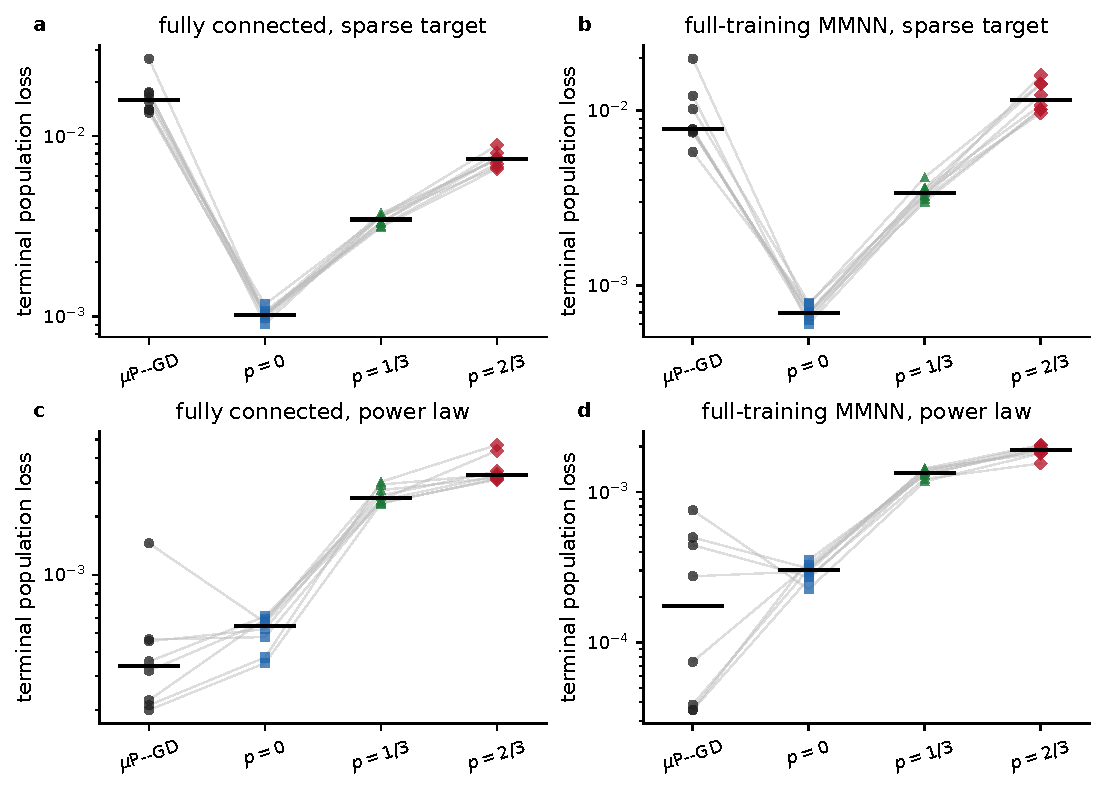
\includegraphics[width=\textwidth]{figures/muon_paired_endpoints.pdf}
 \caption{\textbf{Earlier access is distinct from endpoint dominance.}
 Terminal population losses for the same eight initializations under all
 four update rules.  Gray segments connect paired seeds; colored symbols are
 individual outcomes and black bars are marginal medians.  Rows separate the
 sparse and power-law targets, and columns separate dense and factorized
 networks.  Crossings are retained: a shifted sector clock is not a universal
 terminal-risk ordering.}
 \label{fig:muon-endpoints}
\end{figure}

On the sparse dense target, the gradient-descent clock is
$(25,225,500,{>2500})$ at $q=(1,4,8,16)$.  Polar Muon changes it to
$(50,100,150,325)$.  Muon${}^{1/3}$ gives $(25,50,175,700)$, and
Muon${}^{2/3}$ gives $(25,75,275,1475)$; all spectral medians are observed.

For the MMNN, the four gradient-descent clocks are $25$, $150$, $325$, and
$1500$ steps; polar Muon gives $75$, $125$, $225$, and $450$.  The
fractional powers $p=1/3$ and $p=2/3$ give $(25,75,200,950)$ and
$(25,100,275,2000)$, respectively.  The last value has event coverage
$7/8$.  Thus flattening is not a coordinatewise theorem: it strongly advances
the weak sparse sectors for $p=0$ and $p=1/3$, while $p=2/3$ delays the MMNN
$q=16$ median.

The power-law result is more stringent.  In the dense network, the
$(q=8,16,24)$ gradient-descent clocks $(288,744,1236)$ become
$(132,252,504)$ under polar Muon, with full coverage.  Muon${}^{1/3}$ gives
$(144,468,{>1500})$ and Muon${}^{2/3}$ gives
$(204,732,{>1500})$; their $q=24$ coverages are $3/8$ and $2/8$.
In the MMNN, gradient descent gives $(168,432,564)$, whereas the three
spectral powers give $(180,300,576)$, $(144,384,852)$, and
$(252,684,1092)$.  The descriptive log--log front slopes are respectively
$1.39,.92,1.68,1.86$ in the dense network and
$1.18,.74,1.31,1.51$ in the MMNN, ordered as gradient descent, $p=0$,
$p=1/3$, and $p=2/3$.  Polar Muon flattens the measured front exponent, but
the ideal exponents of \eqref{eq:muon-front-exponent} do not quantitatively
describe all fractional powers.  This is evidence against, rather than an
unreported exception to, literal orthogonal-sector closure.

Endpoint risk reverses the sparse clock advantage on the power-law target.
For sparse targets, the paired median log-loss differences of polar Muon
relative to gradient descent are $-2.72$ in the dense network and $-2.48$ in
the MMNN, with all $8/8$ pairs favoring Muon.  For power-law targets they are
$+.55$ (bootstrap 95\% interval $[.03,.59]$, one win) and $+.78$
($[-.49,2.08]$, three wins), respectively.  Muon${}^{1/3}$ and
Muon${}^{2/3}$ each lose all sixteen power-law endpoint pairs.  The clock effect
is therefore real but is neither a fixed-horizon risk guarantee nor an
optimizer tournament result.

The sparse and power-law panels support the mechanism of
\cref{thm:muon-front}: reducing \(p\) makes weak singular sectors less
subordinate to the leading sector.  They do not validate the orthogonal
closure literally.  In several runs the signed initial velocity of a target
coefficient is negative, and the optimizer ranking changes between dense and
factorized models.  Those are direct signatures of cross-sector and
cross-block coupling omitted from \cref{ass:singular-sectors}.
This separation between an earlier access clock and endpoint dominance also
appears in the twenty-pair three-layer Hermite experiment of
\citet{aiad2026sequential}: spectral updates moved median degree-wise events
earlier, while every paired endpoint interval included zero and event
coverage was equal or lower.  The agreement is mechanistic rather than a
shared asymptotic theorem.
Figure~\ref{fig:muon-endpoints} reports the endpoint estimand separately;
the paired log-loss differences and bootstrap intervals are given in the
machine-readable analysis rather than converted into unpaired error bars.

\begin{figure}[t]
 \centering
 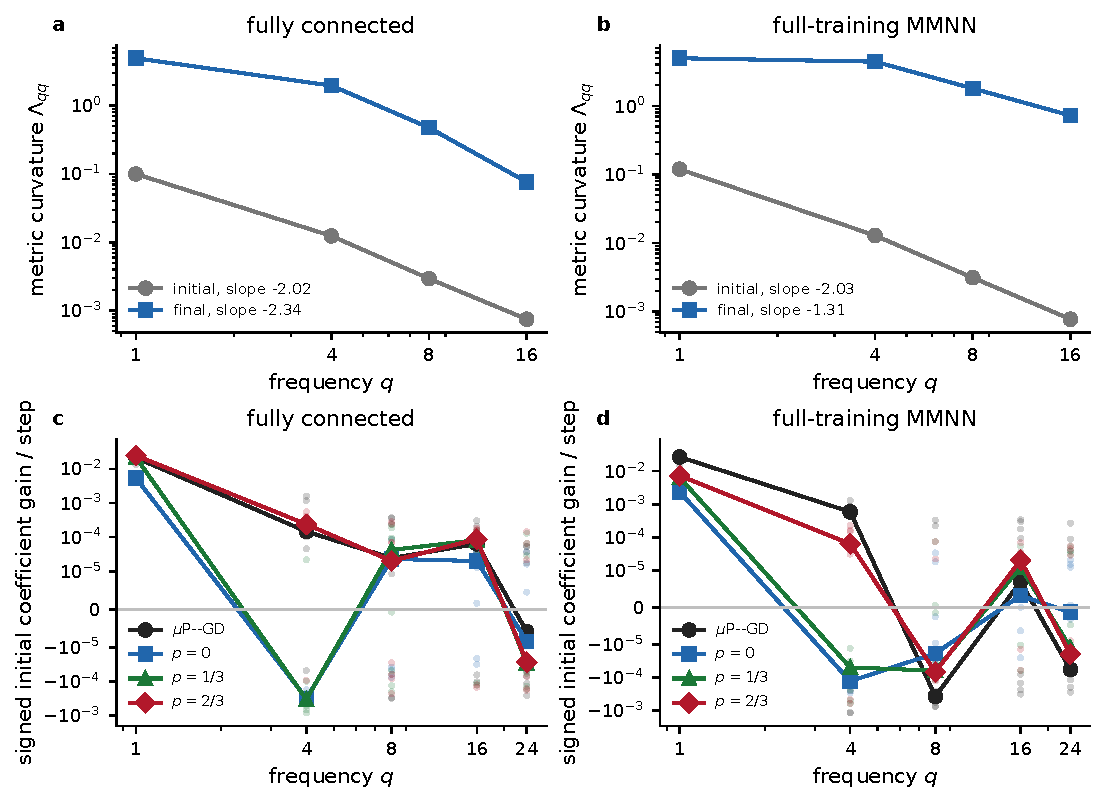
\includegraphics[width=\textwidth]{figures/full_training_dynamic_diagnostics.pdf}
 \caption{\textbf{Dynamic curvature and the failure of a purely diagonal
 Muon picture.}  Top: maximal-update Fourier curvature at initialization and
 the end of full training.  Its prefactor changes by orders of magnitude
 while the high-frequency supply remains decreasing.  Bottom: signed initial
 coefficient gain per optimizer step on the power-law target; faint points
 are paired seeds and lines are medians. Negative values expose cross-mode
 forcing and are retained rather than clipped.}
 \label{fig:full-diagnostics}
\end{figure}

\begin{figure}[t]
 \centering
 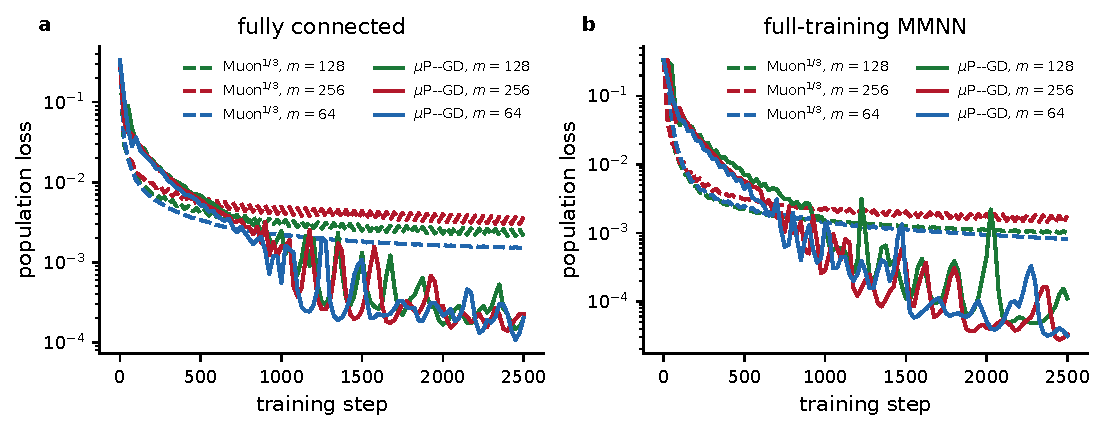
\includegraphics[width=.88\textwidth]{figures/muon_mup_width_transfer.pdf}
 \caption{\textbf{Width transfer without retuning.}  Population loss for
 widths \(64,128,256\) using the learning rate selected at width 128.
 Solid curves are maximal-update gradient descent and dashed curves are
 Muon\({}^{1/3}\).  The comparison is evidence for a common feature-learning
 scale, not a proof of a Muon DMFT.}
 \label{fig:muon-width}
\end{figure}

\begin{figure}[t]
 \centering
 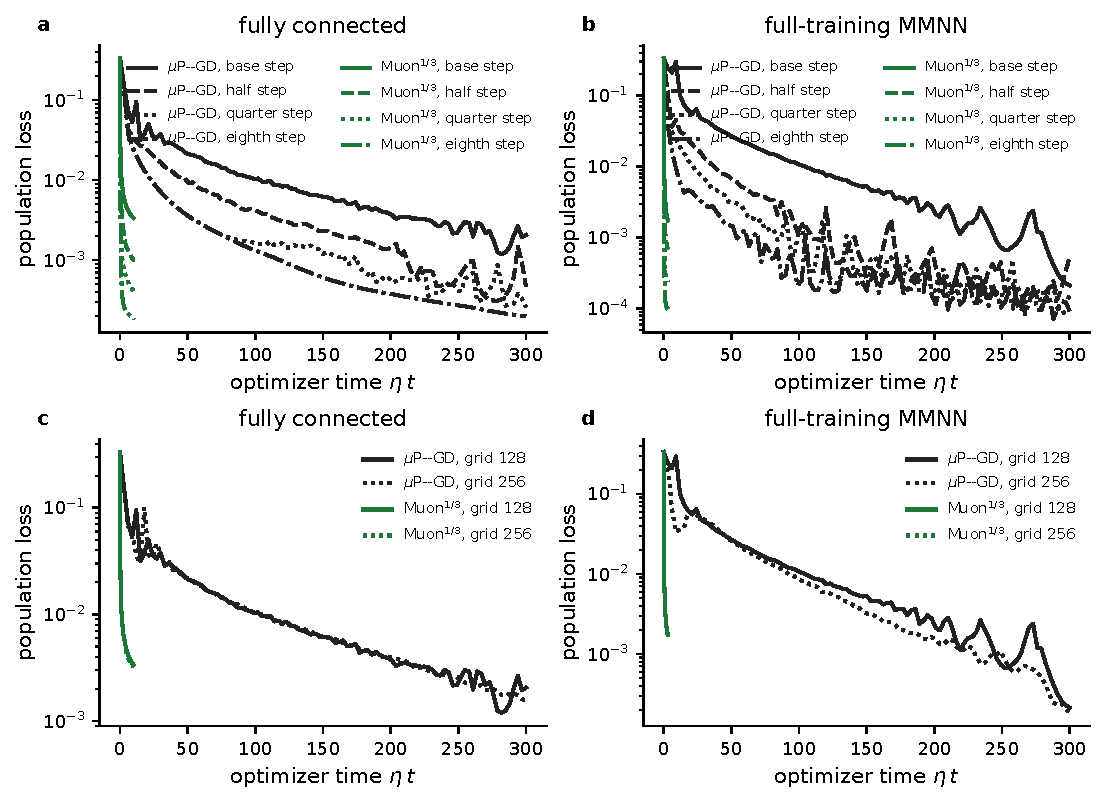
\includegraphics[width=\textwidth]{figures/full_training_step_convergence.pdf}
 \caption{\textbf{Step-size and population-grid controls.}
 Top: the calibrated, half, quarter, and eighth steps, with the horizon
 increased to keep optimizer time $\eta t$ fixed.  Bottom: the 128-point
 population grid is compared with 256 points at the same update rule.
 Curves are medians over three fresh seeds for maximal-update gradient descent
 and Muon${}^{1/3}$; no rate is retuned for a control.}
 \label{fig:discretization}
\end{figure}

Figure~\ref{fig:discretization} is a sensitivity result, not a cosmetic
overlay.  The largest architecture--optimizer median base-to-half change is a
factor $4.11$ in squared population loss.  Because the loss is one half the
squared $L^2$ residual, this is compatible with first-order function error
when the continuum endpoint is small.  From the quarter to the eighth step,
the largest group-median residual-norm ratio is $1.61$; doubling the
population grid changes it by at most $1.33$.  Every base, half, quarter,
eighth, and fine-grid control retains the ordered $q=4,8,16$ clock.
Dense Muon${}^{1/3}$ advances at least one of $q=8,16,24$ in every control;
at the eighth step its $(q=8,16,24)$ clocks are $(320,560,1200)$ updates,
versus $(1280,3360,7120)$ for gradient descent.  The MMNN result is less
uniform: the half-step run has no strict weak-sector advantage, although the
eighth-step clocks $(480,800,1360)$ beat gradient descent
$(400,1200,2320)$ at $q=16,24$ but not at $q=8$.  Thus numerical refinement
supports the hierarchy and the dense speedup, while confirming that the small
MMNN power-law advantage is discretization-sensitive.

The top row of \cref{fig:full-diagnostics} is particularly important for
the NTK objection.  The tangent curvatures change by order one or more under
full training, so the observed clock cannot be generated by freezing the
initial kernel.  The fitted frequency slope can itself change substantially,
as it does in the MMNN.  The bounded-variation theorem is an instantaneous
upper envelope with an evolving budget, not a claim that every finite-range
fit has exponent exactly \(-2\).  The optimizer changes the trajectory
through the nonlinear block map, while regularity continues to constrain the
instantaneous supply of high-frequency tangent features.

\section{Adversarial audit of the claims}
\label{sec:audit}

We record the strongest objections and the corresponding limits of the
result.

\paragraph{``This is still just an NTK proof.''}
No.  The identity \(\dot f=-\mathcal K_t(f-y)\) holds for any differentiable
parameterization.  An NTK proof replaces \(K_t\) by \(K_0\).  We never do so
in \cref{thm:dynamic-saddle}; \(\cB_t\) and \(\Lambda(t)\) may change at
order one.  Empirically, latent motion, gate flips, and frequency-dependent
kernel changes directly reject the frozen-kernel approximation.

\paragraph{``Calling a plateau a saddle is imprecise.''}
Agreed if ``saddle'' means an exact stationary point with a negative Hessian
direction.  Our definition \eqref{eq:saddle-index} is an approximate-saddle
notion: nonzero residual with a parametrically small gradient.  The theorem
proves this notion and no stronger Morse-theoretic claim.

\paragraph{``The residence-time theorem assumes the conclusion.''}
It assumes a quantitative leakage inequality, not sequential learning.  The
inequality is necessary because task adaptation destroys translation
invariance and permits Fourier transfer.  Without it, only the instantaneous
gradient theorem is unconditional.  The measured off-diagonal ratio is
small but nonzero; a fully uniform verification of \eqref{eq:leakage} over
arbitrarily long time remains open.

\paragraph{``A frequency gap should be \(q-p\).''}
The fixed-gap control and \cref{cor:hierarchy} show why this is not an
invariant difficulty measure.  The Fourier integration-by-parts bound sees
\(q\), not a label relative to a previously fitted mode.

\paragraph{``This is precisely the leap framework of
\citet{abbe2023leap}.''}
No.  Their theorem concerns online SGD, high ambient dimension, and new
coordinate support in a tensor-product Hermite/Fourier--Walsh basis.  Our
population circle problem has none of those scaling variables.  More
decisively, \cref{prop:leap-collapse} shows that their definition assigns
the one-coordinate Hermite analogue the minimum degree, independently of
all later frequencies.  What transfers is the sequential-learning metaphor,
not the complexity theorem.

\paragraph{``The result is caused by Adam.''}
No experiment uses Adam.  The geometric campaign uses deterministic
full-batch gradient descent.  The optimizer campaign applies a declared
matrix spectral map, so its difference from gradient descent is the object
being tested rather than an unreported adaptive preconditioner.

\paragraph{``You only confirmed a frozen-left three-map network.''}
That objection applied to the first campaign and motivated the second.  The
full-training study updates every block in dense and factorized networks at
affine depths three, five, and seven.  It confirms the ordering empirically;
\cref{cor:full-depth} supplies the finite-depth theorem.  Neither result is
a uniform-in-depth limit, and the variation-budget constant may worsen with
depth.

\paragraph{``Muon is guaranteed to erase the saddles.''}
False.  \Cref{prop:muon-descent} guarantees total first-order descent, not
positive velocity in every Fourier coefficient.  The clock exponent in
\cref{thm:muon-front} requires biorthogonal singular sectors and controlled
normalization.  Negative measured coefficient velocities and incomplete
event coverage falsify a universal per-mode acceleration claim.

\paragraph{``This is production Muon or an optimizer tournament.''}
It is neither.  We use direct memoryless SVD powers and omit momentum,
Newton--Schulz error, weight decay, and wall-clock matching.  Candidate
learning rates are calibrated on disjoint seeds under a shared protocol,
which makes sector clocks interpretable but does not decide which optimizer
is best under a compute-matched hyperparameter budget.

\paragraph{``Bordelon--Pehlevan DMFT already proves the Muon result.''}
Their self-consistent DMFT proves rich dynamics for the declared
gradient-based computation graph.  A spectral matrix channel is
nonseparable and its response is \eqref{eq:frechet-normalized}.  Reused-data
training additionally generates retarded memory.  The joint Muon closure is
conditional here and in \citet{aiad2026sequential}; width transfer is only an
empirical check.

\paragraph{``Forming $G^\top G$ is numerically equivalent to a direct SVD.''}
Not for the polar member in single precision.  The Gram construction squares
the condition number and, in our audit, changed the polar direction
substantially in small singular sectors. Across nine representative square
gradient blocks, its median cosine with the direct polar direction was $.537$
and its median relative error was $.963$.  We therefore exclude those pilot
outputs, use a direct SVD in confirmation, record its numerical-rank
threshold, and regression-test an ill-conditioned matrix.  This numerical
issue matters less as $p$ approaches one but cannot be ignored at $p=0$.

\paragraph{``Low rank means fixed rank.''}
Not in the deterministic DMFT claim.  We use an extensive bottleneck
\(r/m\to\rho<1\).  Fixed rank is explicitly excluded from
\cref{prop:dmft}, though \cref{thm:factorization} and
\cref{thm:dynamic-saddle} remain valid at finite rank.

\paragraph{``The experiment proves the DMFT equations.''}
It does not.  Width collapse and concentration of measured order parameters
validate predictions of the established wide-limit framework in this
architecture.  A direct numerical solution of the full two-time response
equations would be a stronger comparison.

\paragraph{``HCIZ should produce the saddle hierarchy.''}
HCIZ controls a static rotational integral in a proportional Bayesian
teacher--student problem.  It does not provide the training-time kernel
\(G_t\) of our quenched, masked gradient flow.  Importing it would add
machinery without closing the required dynamics.

\section{Discussion}

The source of the observed frequency leaps is a product of geometry,
dynamics, and optimizer geometry.  Bounded-variation tangent features have
Fourier coefficients of order at most \(1/q\), so scalar-metric curvature is
at most order \(1/q^2\).  In the lazy regime this scarcity persists because
the kernel is fixed.  In masked \(\mu\)P, DMFT evolves the back-propagated
gate kernel; in full training, every forward and backward two-time field
evolves.  A gradient-flow plateau ends by diagonal amplification or
off-diagonal transfer.  A Muon step adds a third route: it flattens the
singular spectrum of the complete matrix gradient, giving weak aligned
sectors more update mass before the tangent kernel has itself adapted.

This distinguishes four statements that are often conflated:

\begin{enumerate}[leftmargin=2em]
\item A tangent-kernel identity is exact for all gradient flows.
\item A frozen tangent kernel is an NTK approximation.
\item A deterministic, evolving tangent kernel is a DMFT order parameter in
the rich infinite-width limit.
\item A nonlinear spectral update is not described by that kernel alone; its
DMFT also needs the Fr\'echet response of the matrix channel and retarded
memory.
\end{enumerate}

Our regularity theorem uses the first, rejects the second, and interprets the
third.  The Muon analysis addresses the fourth under an explicit singular
sector closure.  The resulting hierarchy is robust to feature learning, but
its residence times are not universal because the tangent fields, singular
frames, and cross-mode forcing are task- and architecture-dependent.

The full-training experiments resolve the first obvious extension: freeing
the readout and both MMNN factors changes constants but does not remove the
hierarchy.  The next theoretical target is a direct numerical solution of
the deep two-time DMFT, followed by the nonseparable Muon response closure.
Smooth activations replace the bounded-variation exponent by a higher
Sobolev exponent, yielding steeper scarcity unless feature learning creates
finer scales.  Literal nonnegative factorization requires projected dynamics
and active-set order parameters.  Finally, connecting Fourier plateaux to
the high-dimensional coordinate leaps of \citet{abbe2023leap} requires a
joint target with both support discovery and within-support oscillation;
neither theory alone implies the other.

\section{Conclusion}

Frequency learning in the feature-learning regime is not ``just an NTK
proof,'' and it is not an instance of coordinate leap complexity.  Across
masked and fully trained dense and factorized networks, the kernel and
features move at order one while instantaneous tangent regularity continues
to make high Fourier modes scarce.  This produces a hierarchy of dynamic
approximate saddles.  Gradient-flow DMFT governs whether learned fields build
the missing tangent features or suppress them.  Spectral-power descent can
advance a weak Fourier front by reducing the power with which small singular
sectors are penalized, but cross-sector forcing prevents a universal
per-mode or endpoint guarantee.  The correct conclusion is therefore
mechanistic rather than promotional: feature learning controls the supply of
Fourier directions; Muon controls how the currently supplied matrix-gradient
directions share an update.

\begingroup
\raggedright
\bibliographystyle{plainnat}
\bibliography{references}
\endgroup

\appendix

\section{Further derivations}

\subsection{Fourier coefficient conventions}

For \(u\in L^2(\T)\), write
\[
 u=u_0+\sum_{q\ge1}(u_q^ce_q^c+u_q^se_q^s),\qquad
 e_q^c=\sqrt2\cos(qx),\quad e_q^s=\sqrt2\sin(qx).
\]
The experiment reports the conventional cosine amplitude
\(\widehat u_q^c=2\ip{u}{\cos(q\cdot)}=\sqrt2u_q^c\).  The tangent
curvature in the code includes the factor \(1/2\) needed to convert its
gradient to the normalized coefficient \(u_q^c\).

\subsection{A leakage-free invariant subspace}

If \(K_t(x,x')=\kappa_t(x-x')\) for all \(t\), Fourier modes diagonalize the
kernel and \(\varepsilon=0\) in \cref{ass:leakage}.  In that special case
\[
 R_q(t)=R_q(0)\exp\left(-\int_0^t\Lambda_{qq}(s)\dd s\right).
\]
This formula is exact and non-kernel when \(\Lambda_{qq}(s)\) evolves.  We do
not use it in the main theorem because a fixed cosine target generally
breaks translation invariance of the learned kernel.

\subsection{Approximate purity}

Suppose \(R=Ae_q+\delta\).  Then
\[
 \norm{\nabla\cL}_{\gamma^2nI}
 \leq |A|\sqrt{\Lambda_{qq}}
 +\sqrt{\ip{\delta}{\mathcal K_t\delta}}.
\]
Thus \cref{thm:dynamic-saddle} is stable to a residual perturbation whose
kernel energy is small relative to \(A^2\Lambda_{qq}\).  An \(L^2\)-small
perturbation alone is insufficient if it lies in a very high-curvature
direction.

\section{Reproducibility}

The executable entry point is
\begin{verbatim}
uv run python experiments/mup_dmft_frequency/run_study.py
\end{verbatim}
It writes raw training traces, run summaries, instantaneous Fourier matrices,
metadata, and all figures.  The plotting stage can be repeated without
training using \verb|--plots-only|.  A short end-to-end smoke test is
available through \verb|--quick|.  The implementation automatically uses a
CUDA device when available and otherwise runs on CPU.  Random seeds,
parameterization constants, widths, ranks, time steps, and target amplitudes
are recorded in the output files.

The full-training and spectral-power campaign is reproduced by
\begin{verbatim}
uv run python experiments/mup_dmft_frequency/run_full_training_muon.py \
  --mode calibrate
uv run python experiments/mup_dmft_frequency/run_full_training_muon.py \
  --mode campaign
uv run python experiments/mup_dmft_frequency/run_full_training_muon.py \
  --mode discretization
uv run python experiments/mup_dmft_frequency/run_full_training_muon.py \
  --mode discretization-quarter
uv run python experiments/mup_dmft_frequency/run_full_training_muon.py \
  --mode discretization-eighth
uv run python experiments/mup_dmft_frequency/audit_spectral_backend.py
uv run python experiments/mup_dmft_frequency/sync_full_training_figures.py
# rebuild main.pdf here using the commands above
uv run python experiments/mup_dmft_frequency/audit_full_training_results.py \
  --require-discretization
\end{verbatim}
Calibration and confirmation use disjoint seeds.  The second command writes
all paired trajectories, event summaries, width controls, a JSON claim
analysis, and the additional figures. The third command halves the optimizer
step at matched optimizer time and doubles the population-grid resolution;
the fourth and fifth append quarter- and eighth-step refinements after
inspecting the declared base-to-half and half-to-quarter sensitivities.  The
sixth reproduces the rejected Gram-backend comparison, the seventh
synchronizes vector figures into the paper tree, and the final command fails
closed on the predeclared numerical gates after rebuilding the PDF. A smoke
campaign is available by adding \verb|--quick| to both training stages;
\verb|--mode plots-only| regenerates the figures and analysis without
training.

\end{document}
